\documentclass[tikz,border=3mm]{standalone}
\usepackage{tikz}
\usetikzlibrary{angles,quotes,calc,intersections}
\begin{document}
% TikZ 1
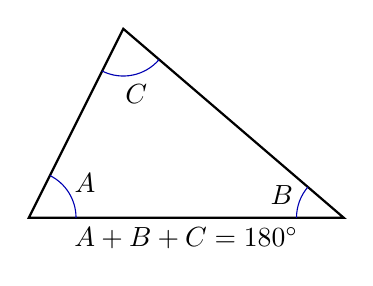
\begin{tikzpicture}[scale=1]
\coordinate (A) at (0,0); \coordinate (B) at (4,0); \coordinate (C) at (1.2,2.4);
\draw[thick] (A)--(B)--(C)--cycle;
\pic[draw=blue!70!black, "$A$", angle radius=6mm, angle eccentricity=1.4] {angle=B--A--C};
\pic[draw=blue!70!black, "$B$", angle radius=6mm, angle eccentricity=1.4] {angle=C--B--A};
\pic[draw=blue!70!black, "$C$", angle radius=6mm, angle eccentricity=1.4] {angle=A--C--B};
\node[below] at (2,0) {$A+B+C=180^{\circ}$};
\end{tikzpicture}
\hspace{1cm}
% TikZ 2
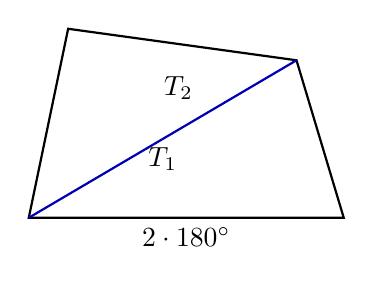
\begin{tikzpicture}[scale=1]
\coordinate (A) at (0,0); \coordinate (B) at (4,0); \coordinate (C) at (3.4,2); \coordinate (D) at (.5,2.4);
\draw[thick] (A)--(B)--(C)--(D)--cycle;
\draw[blue!70!black,thick] (A)--(C);
\node at (1.7,.75) {$T_1$};
\node at (1.9,1.65) {$T_2$};
\node[below] at (2,0) {$2\cdot180^{\circ}$};
\end{tikzpicture}

\vspace{1cm}

% TikZ 3
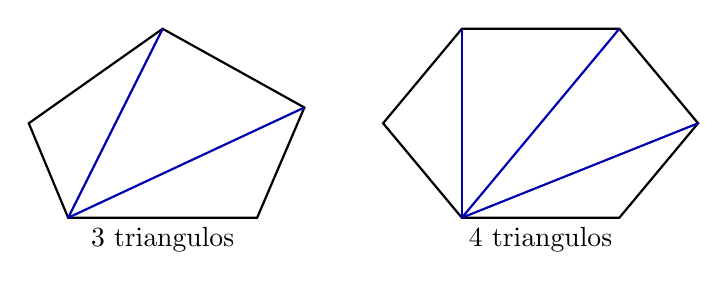
\begin{tikzpicture}[scale=1]
\coordinate (A) at (0,0); \coordinate (B) at (2.4,0); \coordinate (C) at (3,1.4); \coordinate (D) at (1.2,2.4); \coordinate (E) at (-.5,1.2);
\draw[thick] (A)--(B)--(C)--(D)--(E)--cycle;
\draw[blue!70!black,thick] (A)--(C);
\draw[blue!70!black,thick] (A)--(D);
\node[below] at (1.2,0) {3 triangulos};
\coordinate (F) at (5,0); \coordinate (G) at (7,0); \coordinate (H) at (8,1.2); \coordinate (I) at (7,2.4); \coordinate (J) at (5,2.4); \coordinate (K) at (4,1.2);
\draw[thick] (F)--(G)--(H)--(I)--(J)--(K)--cycle;
\draw[blue!70!black,thick] (F)--(H);
\draw[blue!70!black,thick] (F)--(I);
\draw[blue!70!black,thick] (F)--(J);
\node[below] at (6,0) {4 triangulos};
\end{tikzpicture}
\hspace{1cm}
% TikZ 4
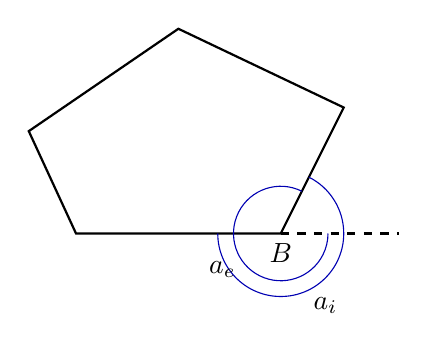
\begin{tikzpicture}[scale=1]
\coordinate (A) at (0,0); \coordinate (B) at (2.6,0); \coordinate (C) at (3.4,1.6); \coordinate (D) at (1.3,2.6); \coordinate (E) at (-.6,1.3); \coordinate (X) at (4.1,0);
\draw[thick] (A)--(B)--(C)--(D)--(E)--cycle;
\draw[thick,dashed] (B)--(X);
\pic[draw=blue!70!black, "$a_i$", angle radius=8mm, angle eccentricity=1.35] {angle=A--B--C};
\pic[draw=blue!70!black, "$a_e$", angle radius=6mm, angle eccentricity=1.45] {angle=C--B--X};
\node[below] at (B) {$B$};
\end{tikzpicture}
\end{document}
